\documentclass[border=10pt]{standalone}
\usepackage[svgnames]{xcolor}
\usepackage{amsmath}
\usepackage{pgfplots}
\pgfplotsset{compat=newest}
\usepackage[sfdefault]{FiraSans}
\usepackage{FiraMono}
\renewcommand*\familydefault{\sfdefault}
\begin{document}
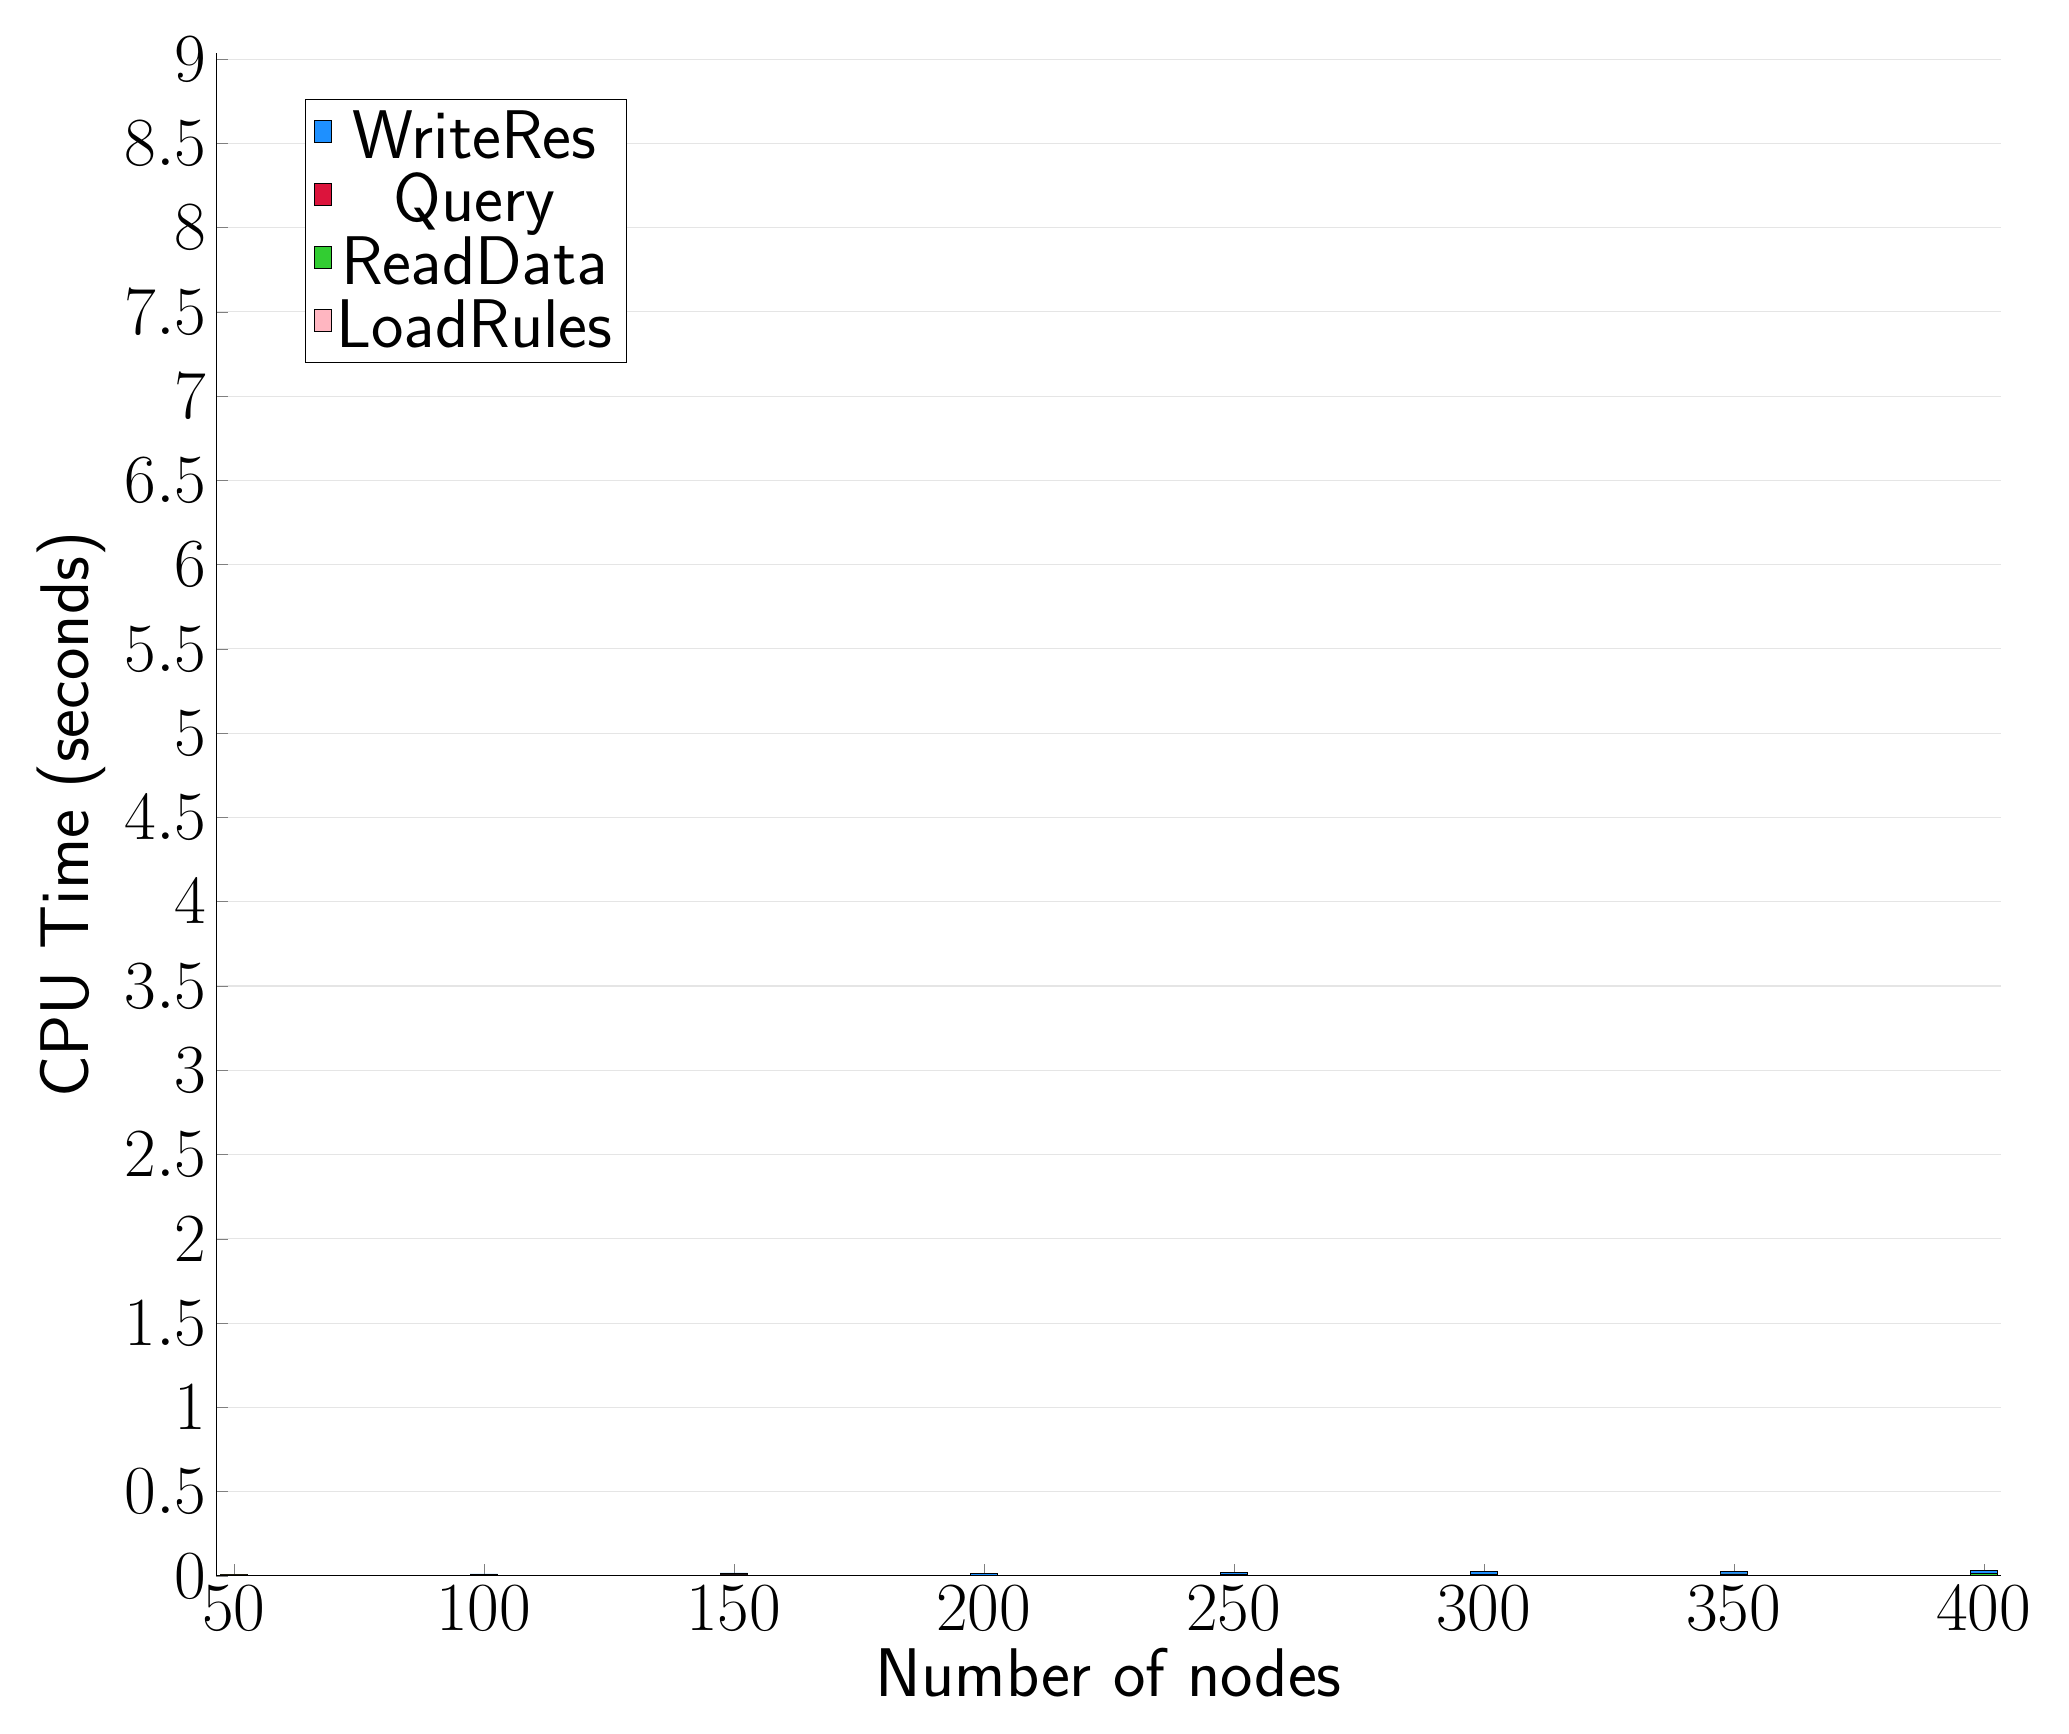
\begin{tikzpicture}
\begin{axis}[
   ybar stacked,
   width=2\textwidth,
   bar width=0.35cm,
   ymajorgrids, tick align=inside,
   major grid style={draw=gray!20},
   xtick=data,
   ymin=0, ymax=9.033333333830038,
   axis x line*=bottom,
   axis y line*=left,
   enlarge x limits=0.01,
   legend style={
       at={(0.23, 0.97)},
       anchor=north east,
       legend columns=1,
       font=\Huge,
   },
   ylabel={CPU Time (seconds)},
   xlabel={Number of nodes},
   label style={font=\Huge},
   tick label style={font=\Huge},
]
\addlegendimage{fill=DodgerBlue, draw=black, line width=0.2pt}
\addlegendentry{WriteRes}
\addlegendimage{fill=Crimson, draw=black, line width=0.2pt}
\addlegendentry{Query}
\addlegendimage{fill=LimeGreen, draw=black, line width=0.2pt}
\addlegendentry{ReadData}
\addlegendimage{fill=LightPink, draw=black, line width=0.2pt}
\addlegendentry{LoadRules}
\addplot +[fill=LightPink, draw=black, line width=0.2pt] coordinates {
(50, 0.005040666666666666)
(100, 0.0044600000000000065)
(150, 0.005910000000000003)
(200, 0.0021236666666666635)
(250, 0.004640666666666667)
(300, 0.0043033333333333335)
(350, 0.004474)
(400, 0.004767666666666663)
};
\addplot +[fill=LimeGreen, draw=black, line width=0.2pt] coordinates {
(50, 0.0013540000000000004)
(100, 0.0024589999999999963)
(150, 0.0037409999999999965)
(200, 0.0026826666666666696)
(250, 0.004645666666666667)
(300, 0.005266333333333341)
(350, 0.006998999999999997)
(400, 0.007763)
};
\addplot +[fill=Crimson, draw=black, line width=0.2pt] coordinates {
(50, 2.733333333333293e-05)
(100, 5.033333333332817e-05)
(150, 6.99999999999983e-05)
(200, 6.266666666666686e-05)
(250, 8.43333333333321e-05)
(300, 9.633333333333256e-05)
(350, 0.0001076666666666702)
(400, 0.00020833333333333335)
};
\addplot +[fill=DodgerBlue, draw=black, line width=0.2pt] coordinates {
(50, 0.0011273333333333337)
(100, 0.005091000000000005)
(150, 0.008500333333333335)
(200, 0.010977)
(250, 0.009643)
(300, 0.014909)
(350, 0.01493133333333333)
(400, 0.020601666666666667)
};
\end{axis}
\end{tikzpicture}

\end{document}
